	\documentclass[
    headings=small,
    version=first,
	oneside,        					% print only on the right pages
    listof=totoc,version=first,     		% includes list of figures and list of tables in table of contents
    bibliography=totoc,version=first,   % includes bibliography in table of contents 
    headsepline,    					% divide under the topline
    12pt
    ]{scrbook}


\usepackage{natbib}

\usepackage{a4}  
\usepackage[left=3cm,right=3cm,top=3cm,bottom=2.5cm]{geometry}
\usepackage[english, ngerman]{babel}
\usepackage[utf8]{inputenc} %damit k{\"o}nnen Umlaute ganz normal geschrieben werden. 
\usepackage{indentfirst}  %Formatter 
\setlength{\parindent}{1cm} 
\usepackage{listings} %Fuer Codelistings

\usepackage{subfigure} %f{\"u}r mehrteilige Grafiken
\usepackage{epsfig}    %damit funktioniert das einbinden von grafiken {\"u}ber epsfig.
\usepackage{graphicx}     % zum einbinden von grafiken
\graphicspath{{grafiken}{../}{kapitel}}
\usepackage{tabularx} 
\usepackage{multirow}    
\usepackage{longtable}	
\usepackage{rotating}	%enable landscape pages
\usepackage{framed}
\usepackage{scrlayer-scrpage}     % paket f{\"u}r kopf- und fu{\ss}zeilen
\pagestyle{scrheadings}   % kopzeilenseitenstil

\usepackage{float} % adds location parameter [H] to [htb] to force figures and tables to a location, no floating
\usepackage{setspace}
\usepackage{url}          % fuer urls: schreibweise ist z.B. \url{http://www.uni-mannheim.de}
\usepackage{nomencl} % um Abkürzungen aufzunehmen: \abbrev{PDA}{personal digital assistant}
\let\abbrev\nomenclature
\renewcommand{\nomname}{List of Abbreviations} %Titel der Liste hier ändern, eine von zwei Optionen nutzen
%\renewcommand{\nomname}{Abkürzungsverzeichnis} %Titel der Liste hier ändern, eine von zwei Optionen nutzen
\setlength{\nomlabelwidth}{.25\hsize}
\renewcommand{\nomlabel}[1]{#1 \dotfill}
\setlength{\nomitemsep}{-\parsep}
\makenomenclature
\newcommand{\Listofabbrev}{
\printnomenclature
\newpage
}




%Inhaltsverzeichnis
\usepackage{tocstyle}			%mehr Kontrolle ueber Inhaltsverzeichnis
\usetocstyle{allwithdot}	%ensure there are dots in table of contents, alternativ: noonewithdot, nopagecolumn
% docu http://www.tug.org/texlive/devsrc/Master/texmf-dist/source/latex/koma-script/tocstyle.dtx
\setcounter{secnumdepth}{3} %numbering up to fifth level in table of contents
\setcounter{tocdepth}{3} %show entries in toc up to fifth level (subsubsubsubsection)


\setlength{\parskip}\medskipamount % Abstand neuer Absatz, besser als explizite Angabe in pt
\onehalfspacing %Zeilenabstand 1,5


\setkomafont{sectioning}{\normalfont\normalcolor\bfseries}

% gestaltung der kopfzeilen
\ohead{\pagemark}
\ifoot{}
\cfoot{}
\ofoot{} 
\cohead{}
\ihead{\headmark}
\setkomafont{pagehead}{\normalfont\bfseries}
\setkomafont{pagenumber}{\normalfont\bfseries}
\automark{chapter}
\automark*{section}


\usepackage{chngcntr}
\counterwithout{figure}{chapter}
\counterwithout{table}{chapter}




% ----- ende der pr{\"a}ambel ----------------------------------






\begin{document}  % dokument f{\"a}ngt an
\selectlanguage{english} %englische Silbentrennung, fuer deutsche Arbeiten: \selectlanguage{ngerman}
\frontmatter      % vorspann, kapitel r{\"o}misch nummeriert

\newgeometry{margin=3cm}
% Die Titelseite der Arbeit

\begin{titlepage}

\begin{center} % zentrieren

  % Logo
  \begin{figure}[ht]
    \centering
    
\includegraphics[width=.5\textwidth]{grafiken/unilogo.png}
  \end{figure}
  
  % Vertikaler Zwischenraum
  \bigskip
  \vfill 
  \begin{framed}
    \begin{center}
     \textsc{{\LARGE Thesis title}}  \\
      \bigskip
	%Here goes the subtitle
      SUBTITLE\\
      \bigskip
      \textbf{Master Thesis}
    \end{center}
   \end{framed}
    \vfill
    \vfill
  
%Students Data
  \begin{tabular*}{0.62\textwidth}{r@{\extracolsep{\fill}}l}
   Submitted: &\hspace{1cm} December 2020\\\\
   By: &\hspace{1cm} Cara Maria Damm\\
		&\hspace{1cm}  cadamm@mail.uni-mannheim.de\\
    &\hspace{1cm} born June 18 1994\\
    & \hspace{1cm} in Karlsruhe, Germany\\
    \\
    Matriculation Number: &\hspace{1cm} 1631263\\
    \\
     Supervisor: & \hspace{1cm} Philipp Hoffmann\\
     Reviewer: &\hspace{1cm} Prof. Dr. Armin H. Heinzl\\

  \end{tabular*}
    
  \vfill
  \vfill

  
  \rule{\textwidth}{.4pt}\\ % vertikale Linie
  University of Mannheim\\
  Chair of General Management and Information Systems\\
 68131 Mannheim\\
  Phone: +49 (0) 621 181 1691, Fax: +49 (0) 621 181 1692\\
  Homepage: https://www.bwl.uni-mannheim.de/heinzl/
\end{center}

\end{titlepage} 
%//End of Title

 
     % titelseite einbinden
\restoregeometry



\chapter{Abstract}
\thispagestyle{empty}

The abstract offers a brief description of your thesis and a concise summary of its conclusions. Be sure to describe the subject and focus of your work. Please avoid symbols, foreign words, formulas, diagrams and other illustrative materials, lengthy explanations, or opinions. Do not exceed 200 words.

\tableofcontents            % inhaltsverzeichnis

\listoffigures              % abbildungsverzeichnis
\listoftables               % tabellenverzeichnis


\addcontentsline{toc}{chapter}{\nomname} %abkuerzungen ins inhaltsverzeichnis

\Listofabbrev % liste der abkuerzungen erstellen



\mainmatter       % hauptteil, kapitel lateinisch nummeriert
\include{chapter/content}
\chapter{Introduction}

This exemplary document serves as a guideline for both the outline and format of your work. In this section, you introduce the topic. The research problem should be derived from real-world situations and research to show awareness of the issue. Therefore, you should present the business problem, the scientific problem, the paper’s objectives, and the expected contributions. A good guideline on the content and structure of a research paper is provided by Venkatesh (2011, pp. 46–54) \citet{tannenbaum}. In the following chapter, the citation style for your thesis will be explained and presented. Here comes a change

\section{Objectives of the Thesis}
In order to create a common understanding of the research project described in your thesis, it is important to highlight the objectives of this thesis. The formulation of research questions is helpful to conclude the objectives in a concrete manner.
\section{Structure of the Thesis}
The explanation of the structure of your thesis helps a reader to follow your concept and offers a rough overview of the chapters of your thesis.
\chapter{Theoretical Foundation}

If your work is based on other scientific theories and models, it is important to outline their structure and results. Use illustrations of models and theories as demonstrated below in Figure \ref{fig1}

\begin{figure}[H]
\centering
  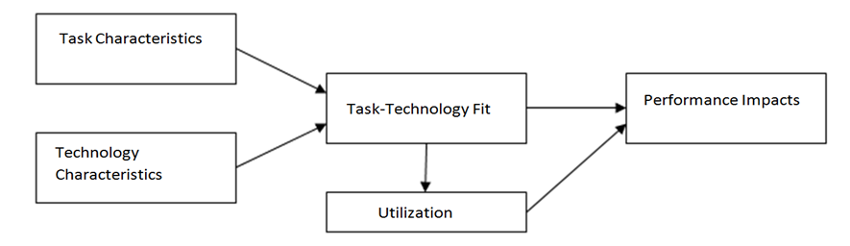
\includegraphics[width=0.5\textwidth]{grafiken/fig1}
   \caption{A picture of the universe!}
   \label{fig1}
\end{figure}


In addition to figures, one of the most powerful ways to present information in a coherent way is to create tables as shown in \ref{tab:table-name}. Make sure to include an empty line above tables and figures.
\begin{center}
\begin{table}[H]
\begin{tabularx}{\textwidth}{|X|X|X|}
\hline
Input & Output& Action return \\
\hline
DNF &  simulation & jsp\\
\hline
\end{tabularx}
\caption{\label{tab:table-name}Your caption.}
\end{table}
\end{center}


Multiple ways of presenting information can be chosen, e.g.

\begin{list}{•}{}
\item figures,
\item tables,
\item ordered lists,
\item and enumerations like this one. Here, items can be single sentences or full paragraphs. Appropriate end punctuation should be included.

\end{list}


\include{chapter/chapter3}
\include{chapter/chapter4}
\include{chapter/chapter5}
\include{chapter/chapter6}

\selectlanguage{english} % jetzt sprechen wir wieder englisch
\backmatter
\pagenumbering{roman}
\setcounter{page}{7}

%Bibliographie
%waehle einen der folgenden 4 Eintraege
%\bibliographystyle{literatur/natdin} %DIN Style Literaturverzeichnis, comment out pagebackref
%\bibliographystyle{literatur/IEEEtran} % IEEE Style Literaturverzeichnis
%\bibliographystyle{literatur/natdinCustomized} %DIN Style Literaturverzeichnis + Punkt hinter jeder Literaturangabe -> low level config fuer Zitate: natdin.cfg im Projektordner, comment out pagebackref

%\bibliographystyle{literatur/natdinCustomizedEnglish} %DIN Style auf Englisch getrimmt mit Punkt hinter Literaturangabe -> low lovel config fuer Zitate: natdin.cfg im Projektordner, pagebackref kann damit nicht genutzt werden
%\bibliographystyle{aer} % alternativ auch apalike, aer, apalike2... s.a. http://web.reed.edu/cis/Help/LaTeX/bibtexstyles.html
%\bibliographystyle{plain} % very nice bib style
%note on aer: does not like inbook entries
%\bibliographystyle{natdin}
\bibliographystyle{literatur/apa-good}

\bibliography{literatur/lit} %Pfad zur bib-Datei

%appendices can be defined here, the appendix structure has to be added manually to the toc (table of contents)
%\clearpage  %toc new page
%\addcontentsline{toc}{chapter}{Appendix} %add chapter to toc

%\addpart{\appendixname}
\chapter{}

\section*{Appendix A}

Appendices contain any further information, which is noteworthy but not necessarily needed to describe in the main part of your thesis. Often complex tables and figures created during your research project will be presented in an Appendix




%Eidesstattliche Erklaerung
\chapter*{\large Affidavit}
\pagestyle{empty}
I hereby declare that I have developed and written the enclosed master thesis entirely on my own and have not used outside sources without declaration in the text. Any concepts or quotations applicable to these sources are clearly attributed to them. This  master thesis has not been submitted in the same or a substantially similar version, not even in part, to any other authority for grading and has not been published elsewhere. This is to certify that the printed version is equivalent to the submitted electronic one. I am aware of the fact that a misstatement may have serious legal consequences.\\

I also agree that my thesis can be sent and stored anonymously for plagiarism purposes. I know that my thesis may not be corrected if the declaration is not issued.


\vspace{2.0cm}

Mannheim\\
\vspace{1cm}
\hspace{0.1cm} \today



\vspace{2cm}
Max Mustermann



\end{document}
